\documentclass{article}

\usepackage{amsmath}
\usepackage{graphicx}
\usepackage{courier}
\usepackage{multicol}
\usepackage{microtype} %required to fix courier linebreaking issues
\usepackage{hyperref} % make references into links
\usepackage{amsfonts}
\hypersetup{colorlinks=true, linkcolor=blue} %make them pretty links
\usepackage[all]{hypcap} %make them link to the right place
\usepackage{url}
\makeatletter
\g@addto@macro{\UrlBreaks}{\UrlOrds}
\makeatother
\usepackage{geometry}
\geometry{legalpaper, portrait, margin=1.5in}

\begin{document}
	\title{CS182: NBA Scheduler}
	\author{Abhishek Malali (abhishekmalali@g.harvard.edu)\\
			Charles Liu (cliu02@g.harvard.edu)\\
			Samuel Daulton (sdaulton@g.harvard.edu)}
	\date{\today}
	\maketitle
	
	\section{Introduction}
	
	The National Basketball Association is a 30 team league that organizes an 82 game schedule for each team over a 6-month period. It showcases some of the best athletes in the world and has generated globally recognized brands. As such, it is a multi-billion dollar industry and is constantly looking for ways to improve. Recently, one such way has been to reorganize its schedule.
	
	\subsection{NBA Scheduling Formula}

	Currently there are two conferences (East, West) each comprised of three divisions each of which contain five teams. The 82-game schedule is currently set up as follows:

	\begin{enumerate}
		\item 4 games against the other 4 division opponents, [4x4=16 games]
		\item 4 games against 6 (out-of-division) conference opponents, [4x6=24 games]
		\item 3 games against the remaining 4 conference teams, [3x4=12 games]
		\item 2 games against teams in the opposing conference. [2x15=30 games]
	\end{enumerate}

	And of course, each team must play 41 home and 41 away games. 
	
	\subsection{Court Availability}

	As these are actual games with required venues, each team must provide the following:

	\begin{enumerate}
		\item At least 50 dates on which their home court will be available
		\item 4 Mondays
		\item 4 Thursdays (to help TNT plan its telecasts).
	\end{enumerate}

	\subsection{Official Breaks}

	There are no games on the following days:

	\begin{enumerate}
		\item Christmas Eve
		\item All-Star Week
		\item NCAA Men's Division I Basketball Championship Game
	\end{enumerate}

    \subsection{Additional Assumptions}
    
    There are no non-NBA events in the venues that may further constrain a team's schedule.
	
	\section{Data Generation}

	We created simple classes representing teams, divisions, and conferences mimicking the structure of the league. We also created a data generation (datagen) class that generates a master list of dates - these dates conform to the scheduling requirements mentioned above. In particular, Christmas Eve is obviously December 24, we randomly select a week for an All-Star Break in February and the NCAA Men's Division I Basketball Championship is assumed to be the first Monday of April.

	Once we have our list of dates, we map them to indices ranging from 0 to the number of dates. All our subsequent calculations are based on these numbered indices. For each team, we randomly choose 3-5 dates in every 5-day period as potential home dates. We will discuss the implications of this in our results.
	
	\section{Integer Linear Programming}
	Integer linear programming is a mathematical optimization where all variables are restricted to integers. The objective function and the constraints are linear. In the NBA scheduling problem, the objective function is not defined and the solver has to solve the constraints as formulated in the problem. We solved this problem in 2 steps. The first was to attempt getting a schedule roundwise without considering the dates. Next we included dates and were able to create a player friendly schedule where there no more than 3 games in 5 days.
	
	\subsection{Methodology for the roundwise schedule}
	We create a variable for every team against every other team, for every round. The first part of the variable is the home team followed by the away team and the round number. We introduce the following constraints to the ILP
	\begin{enumerate}
		\item All teams play 82 games, 41 home and away
		\item All constraints for the division, in conference and out of conference teams
		\item No team can play more than one game in a round
		\item Team can only play either home or away
	\end{enumerate}
	The above ILP was solved using the PuLP as well as the GUROBI solver. The PuLP solver took 40 minutes to converge to solution whereas the GUROBI solver took 6 seconds on average. The schedule was verified using tests to check if all constraints were satisfied.
	
	\subsection{Generating the player friendly schedule}
	Using the dates generated by datagen, we formulated the ILP for a player friendly schedule. The variables are created for every date instead of every round.  To reduce the number of variables we generate the variables for every possible home and away dates only. This reduces the number of variables by about 70\%. The time taken to create the constraints and to solve the ILP are greatly reduced. We use the following constraints.
	\begin{enumerate}
		\item All teams play 82 games, 41 home and away
		\item All constraints for the division, in conference and out of conference teams
		\item No team can play more than one game on a single date
		\item Team can only play either home or away
		\item A team can only play 3 or lesser matches in 5 days
		\item A team does not play 2 away games without a day's break
		\item A team does not play an away game right after a home game
	\end{enumerate}
	The above ILP was solved using the PuLP as well as the GUROBI solver. The PuLP solver took 1 hour to converge to solution whereas the GUROBI solver took 29 seconds on an average. In some cases the 4 games in 5 days was unavoidable due to mismatch in dates, but our solution aimed to minimize it.

	\section{Constraint Satisfaction Problem}
	The ILP solution was mainly used as a speed benchmark for us. Although our solution is written in pure Python and the ILP solver most likely uses some C or Fortran bindings, we have the advantage of using heuristics to aid finding a solution.

	We modeled our problem in two sub-CSP's: one for attaining matchups and game numbers ($MSP$), and one using those matchups/game numbers to find suitable home/away and date assignments ($HSP$). The formulation from variable to domain was as follows:

	\begin{eqnarray*}
		MSP: (Team_1, game\_num) &=>& (Team_2) \\
		HSP: (Team_1, Team_2, game\_num) &=>& (Date, True/False)
	\end{eqnarray*}

	The results from $MSP$ formed the variables for $HSP$, with the ordering of the teams assigned lexicographically. An assignment of $True$ in the domain for $HSP$ referred to $Team_1$ having the home game. 

	\subsection{Matchups CSP}
	Within our code, for each team we initialize a list of opposing teams with each team repeated to the number of times these two teams play. Our $MSP$ then will form the unique list of teams from this list to try assignments. 

	\begin{figure}
	\caption{Example of current state during $MSP$. The number next to the opposing team corresponds to the number of games left to play against the Knicks.
	min\_count(Knicks)=1 and sum\_count(Knicks, Celtics)=2}
	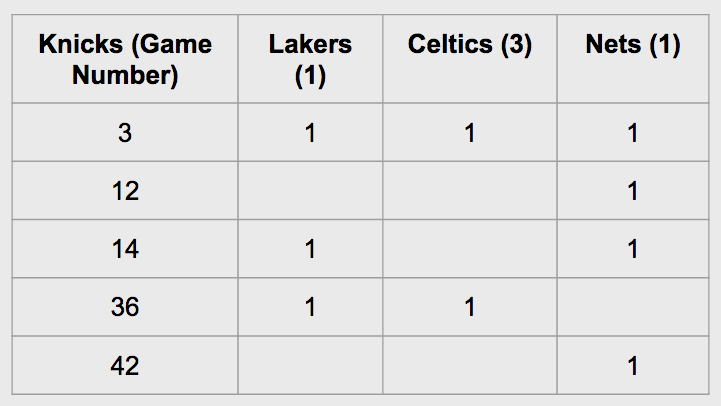
\includegraphics[scale=0.6]{matchups_game_counts}
	\end{figure}

	We define two useful functions for our CSP:
	\begin{itemize}
		\item min\_count($Team$) - minimum row count over remaining games
		\item sum\_count($Team_1, Team_2$) - sum over column for $Team_2$
	\end{itemize}

	\subsubsection{Heuristics}
	There were a number of heuristics we used to solve this CSP.
	\begin{enumerate}
		\item We applied forward checking to each successor state we looked at. This consisted of checking that the min\_count for every team was at least 1 and the sum\_count over every pair of teams was at least as large as the number of games they had left to play.
		\item We chose the next team/game to assign by finding the team with the lowest min\_count and it's associated game.
		\item After choosing $t,g$ for the team/game number to next assign, we ordered the possible opponents using the least-constrained heuristic. This involved trying out the assignment and recalculating min\_count($t$). We then ordered the possible opponents in decreasing order - the opponent that kept the min\_count from dropping the most was the least constrained assignment.
	\end{enumerate}

	\subsubsection{Results}
	The CSP solves typically in 2-3 minutes with around 1600 states explored. The heuristic that was the most valuable was the least-constrained variable heuristic, as without it the CSP would not complete.

	\subsection{Dates/Venues CSP}
	Using the results from the Matchups CSP, we formulated this problem first as a DFS again. In our code, for any pair of teams we stored a list of True/False tuples according to the number of times those two teams played. If the teams played three times, there'd be two Trues and two Falses. We also created a master list of possible dates with the keys being $(Team_1,Team_2,game\_num,True/False)$. This represented the possible dates for any matchup and home/away combination (True meaning $Team_1$ was home). For the home team, let the set of home dates generated in our initial data generation process be $D$. We defined a hyperparameter $window$, and assigned the values to this dictionary as:

	\begin{eqnarray*}
		\forall x \in D: x \geq 2*game\_num - window \land x \leq 2*game\_num + window
	\end{eqnarray*}

	The rationale here is the season is typically 160-170 days, meaning ideally each game is every other day. So, we specify the domain of possible dates for a game to be a window of dates centered at that ideal date. The heuristics used were as follows:
	\begin{enumerate}
		\item Forward checking was relatively straightforward in this CSP. We remove any True/False possibilities for any pair of teams if one team has reached the limit of home or away games for that matchup. For any date $d$ we assign for some game\_num, we remove the dates prior to $d$ for any game after game\_num, and any date after $d$ for any game before game\_num for any matchup involving one of these teams.
		\item Choosing what matchup to next assign was the most perplexing part of this problem. We initially chose the team with the most assignments up to that point - essentially trying to assign all home/away matchups for a specific team at a time. The difficulty in this CSP is finding the right assignments for matchups of teams that play 3 times. There's an added complexity of having the right combination of 1 home/2 away and 2 home/1 away matchups that keep each team's total home/away games even. What was originally happening was the DFS would assign every matchup for every team until the last few, but it was impossible to find a right assignment for them because too many teams had their 3-game matchups with a given 2-home or 2-aways. There wasn't a good backtracking method implemented once that happened, so the CSP would stagnate through all possible iterations. Given that, we decided to first assign all matchups between opponents that play an even number of times and only after all those were completed do we start on the 3-game matchups. This was the key to solving this CSP.
		\item Once we had our matchup we wanted to assign, we checked which values True or False were possible - if a team had reached their limit of home/away games then there was no ordering to be done. If both teams could potentially be the home team, we chose to first try the team with the fewer number of home games be the potential home team. Then, for any Home/Away assignment, we had our master dates list with potential dates. We ordered these according to the distance to the ``ideal date'', the 2*game\_num we had used to first assign the window of possible dates. The resulting list of possible assignments was interleaved True/False assignments with their associated dates based on distance to the ``ideal date''.
		\begin{itemize}
			\item As an example suppose for $(Team_1,Team_2,game\_num=10)$, the window of home dates for $Team_1$ are $(17,19,21,23)$ and the window of home dates for $Team_2$ are $(18,20)$. We want to first try $Team_2$ as the home team because to that point it's had less home assignments, so False would take priority to True. The resulting ordering of the domain would be: (20,False), (19,True), (18,False), (21,True), (23,True), (17,True) - ordering of 19/21 and 17/23 could be flipped based Python's sort implementation.
		\end{itemize}
	\end{enumerate}

	There's potentially no solution to our problem given the availability of home dates. This goes back to our original dates formulation - randomly selecting between 3-5 home dates every 5 days of the season for every team. If every date were possible - i.e. each team's possible home dates were every day of the season, our CSP solves in under a minute with typically under 1000 states explored. If we set the possible home dates to be 3 out of every 5 dates, our CSP solved roughly half the time. This was the rationale for us to randomly choose between 3-5 home dates, as we generally obtain solutions and they're more interesting than a game every other day.

	\subsubsection{$M$ games in $N$ nights}
	We use Dijkstra's algorithm to find a schedule that satisfies the ``no $M$ games in $N$ nights'' soft constraint. For our problem, let $M=4$ and $N=5$
    The algorithm works as follow:
    \begin{enumerate}
    	\item The initial state (where no matchups have been assigned dates or venues), is assigned a cost of 1230 (the number of remaining unassigned matchups). Note that a successor state is the current state with one more matchup assigned a date and home/away.
    	\item Each possible successor state is assigned a cost of $Unassigned + Dist$, where $Unassigned$ refers to the number of total matchups remaining to be assigned (should decrease from 1230 by 1 every time) and $Dist$ is the distance to the ideal date for the new matchup assigned (to retain the date ordering from our heuristics)
    	\item If one team of the new matchup assigned plays at least $M$ games in $N$ nights, a penalty 10000 is added to the cost
    \end{enumerate}
    The cost is used as the priority when adding a state to the frontier priority queue. Again, how we generate the home dates for our teams is crucial to determining the runtime of finding a solution (if it exists). If we give every team a home date for every day of the season, our UCS runs exactly as our previous DFS as every game will be assigned essentially the ideal date. The UCS will explore exactly the same states, but will take a bit longer to run given the added computation of calculating the maximum number of games over any $N$-day period - roughly 2 minutes. Sometimes a season is a little under 164 days, so in that case a solution is found in about 2500 states explored. With the random 3-5 days in any 5-day period, if a solution exists without breaking the soft constraint it will find it in approximately the same time, but if no such solution exists it takes an indefinite amount of time to find a solution. We believe having a good heuristic function would help with this, but were unable to come up with an admissible one that helped.

	\section{Running the Repository}
	We felt it unnecessary to submit the code to Canvas as there are quite a few files. Our github repository is located at \url{https://github.com/chuckyouliu/NBA_Scheduler}. Basic description of important files:

	\begin{itemize}
		\item ILP\_formulation.py - As name suggests the ILP code is located here
		\item datagen.py - Formulation of the date indices
		\item organization.py - Classes corresponding to team/division/league/conference
		\item domain.py - Classes corresponding to the CSP's with functions calculating the heuristics
		\item constraint.py - Functions associated with forward checking, used by classes in domain.py
		\item scheduler.py - Main class for solving schedule, creates variables/domains that are fed into domain.py
	\end{itemize}
	To create a schedule, you can use a command line tool that we've written called write\_schedule. An example command would be:
	\begin{center}
		python write\_schedule.py -m True -d True -y 2016
	\end{center}
	This would create a schedule for the year 2016. The -d stands for debug, so debug outputs would be shown, and the -m stands for if you'd like to use an already existing Matchups.json file, so only create new home/aways and dates not new matchups. Setting that to False would create an entirely new schedule with new matchups.
	Our results of an example schedule are stored in the json files. We created a simple command line tool to read from the json files by typing for example:
	\begin{center}
		python read\_schedule.py -n 5 -t Knicks,Celtics
	\end{center}
	This will output the first 5 games of the schedule for Knicks and Celtics. Use -h to see the list of possible teams.

	\section{Work Distribution}
	\begin{itemize}
	\item Data Generation - Charles created the structure of the league as well as the initial data generation class. As the project progressed changes were made by all members.
	\item ILP - Sam and Abhishek worked on the initial matchups problem. From there, Abhishek took the lead on solving home/away's and dates as well as moving to the faster GUROBI.
	\item CSP - Charles created the general structure of the scheduler/domain/constraint files and the sub-CSP problems. From there the more involved work (heuristics, testing) were split as follows:
		\begin{itemize}
			\item Matchups heuristics - Charles
			\item Home/Aways heuristics - Charles and Sam pair coded
			\item Dates/UCS - primarily Sam with some input on cost functions from Charles
		\end{itemize}
	\end{itemize}
	
\end{document}
